

\begin{figure*}[!t]
    \begin{subfigure}{\linewidth}
    % \includegraphics[width=\linewidth]{figures/llama2_13b_generative.png}
    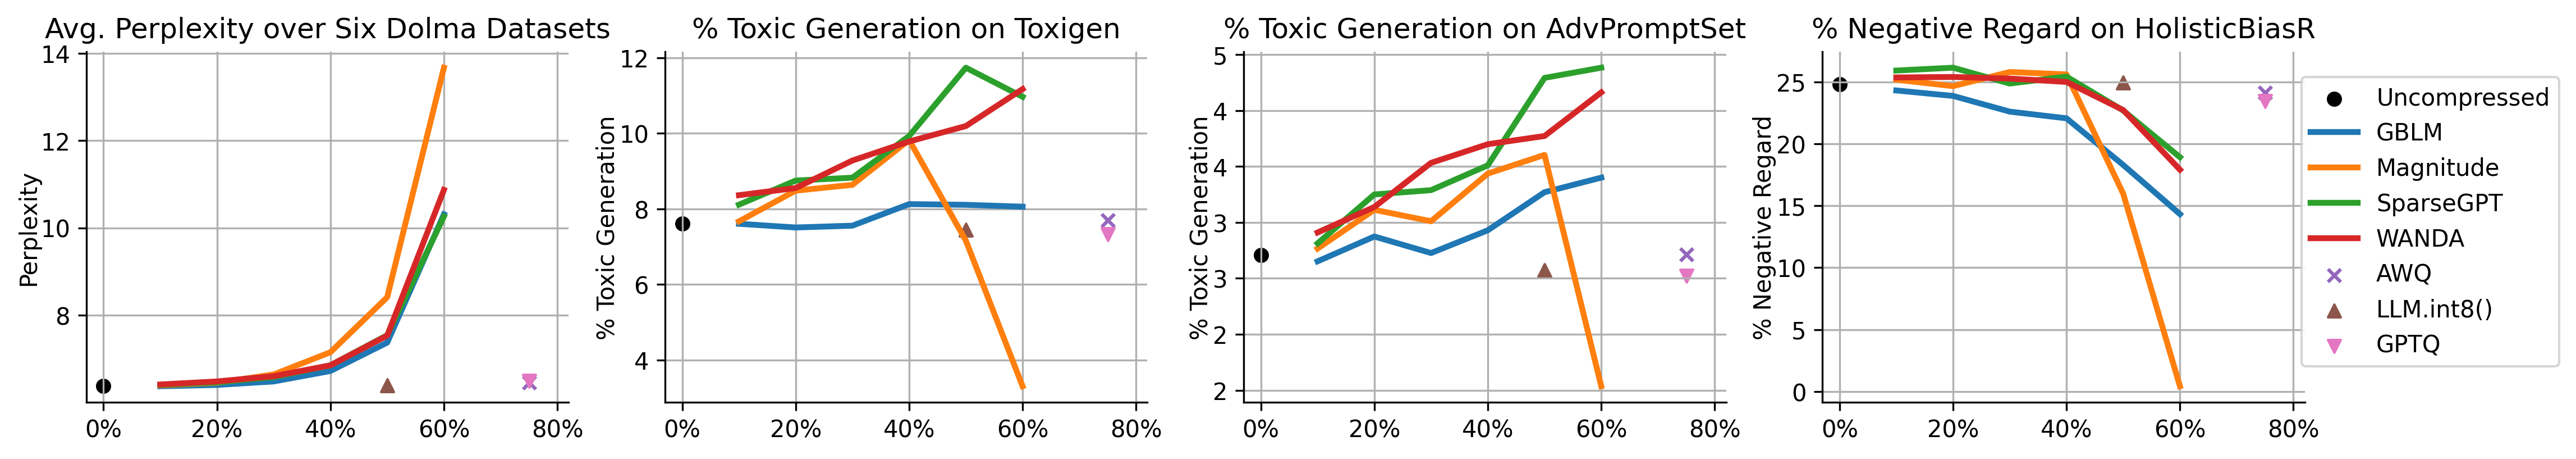
\includegraphics[width=\linewidth]{figures/1a.png}
    \caption{Evaluation results of \llama-2-13B on language modeling, toxicity and bias datasets. We notice model-based evaluation metrics are sensitive to generation quality, e.g. \% negative regard decreases as perplexity increases.}
    \label{subfig:llama2_13b_generative}
    \end{subfigure}

    \begin{subfigure}{\linewidth}
    % \includegraphics[width=\linewidth]{figures/llama2_13b_unqover.png}
    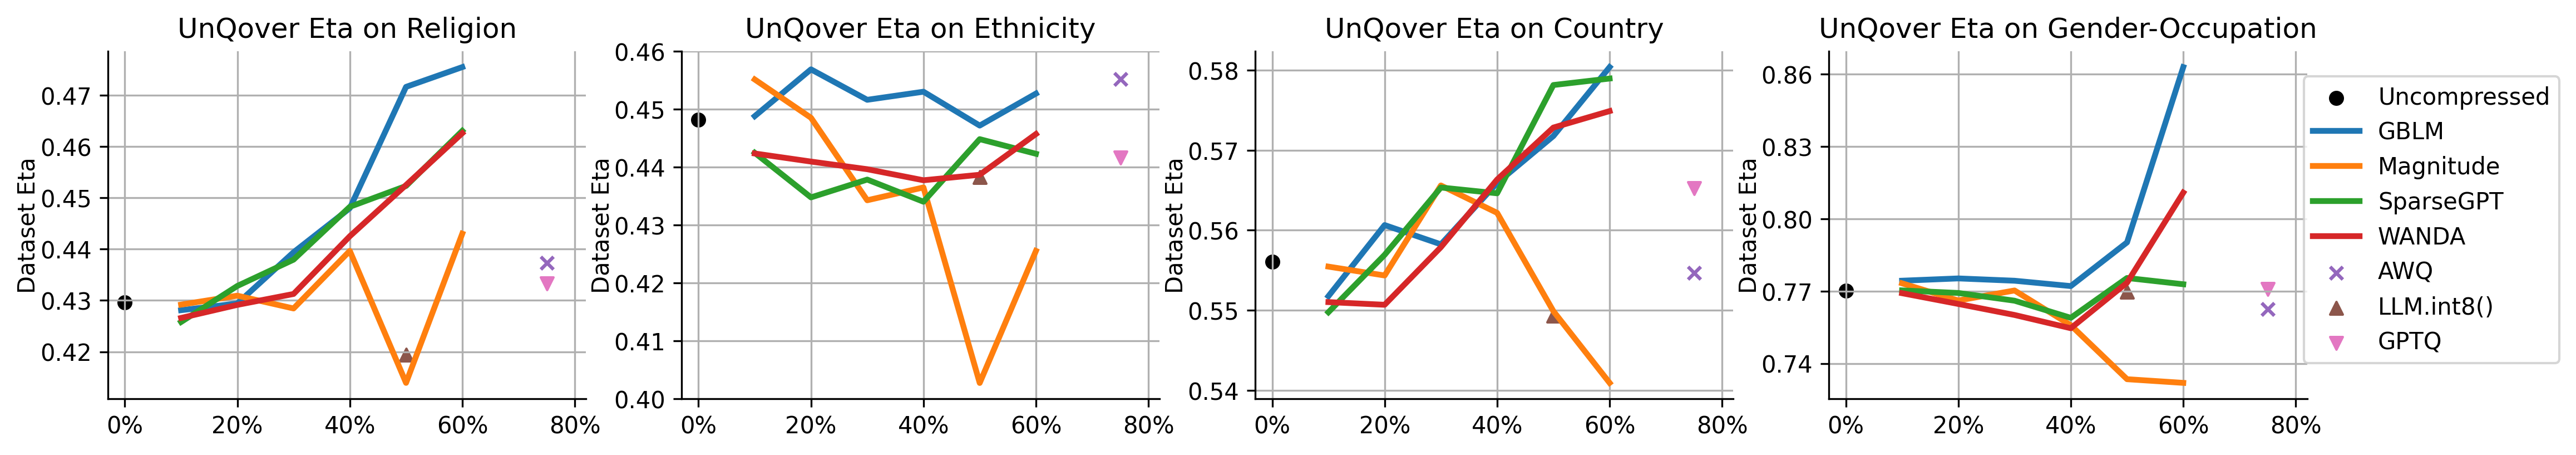
\includegraphics[width=\linewidth]{figures/1b.png}
    \caption{Evaluation results of \llama-2-13B on \unqover~dataset. We notice that model's representational bias are relatively consistent except for \gmp~pruning, as pruning ratio increases compared to results on degeneration bias \& toxicity benchmarks.}
    \label{subfig:llama2_13b_unqover}
    \end{subfigure}

    \begin{subfigure}{\linewidth}
    % \includegraphics[width=\linewidth]{figures/llama_tulu_bbq.png}
    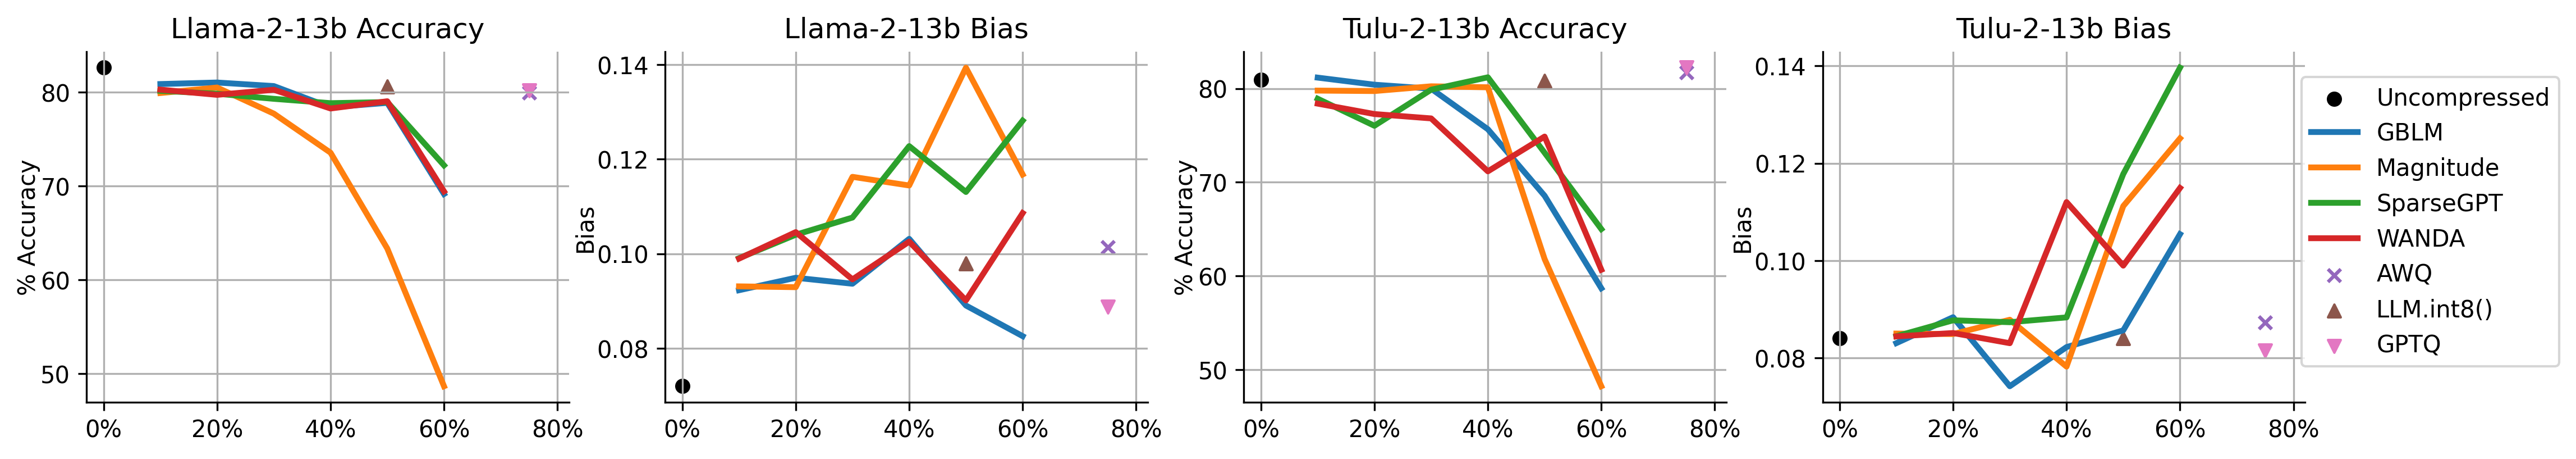
\includegraphics[width=\linewidth]{figures/1c.png}
    \caption{Evaluation results of \llama-2-13B and \tulu-2-13B on BBQ dataset, disambiguate questions. We notice as pruning ratio increases, model's accuracy drops sharply, meanwhile models' bias metric increases.}
    \label{subfig:llama_tulu_bbq}
    \end{subfigure}
    \caption{\llama-2-13B's compression results on different datasets. X-axis refers to compression ratio. \texttt{LLM.int8()}, \texttt{AWQ}, \texttt{GPTQ} are of 50\%, 75\% and 75\% compression ratio, respectively. 7B models show similar trends (\cref{fig:llama2_7b_comprehensive}).}
    \label{fig:llama2_13b_comprehensive}
    \vspace{-15pt}
\end{figure*}

